%************************************************
\chapter{Reflectively Learning to Control}
\label{chapter:reflectively_learning_to_control}
%************************************************

In order to demonstrate my solution to the problem of reflectively
learning-to-control, I will focus on a running example within the
physical block building domain shown in
\autoref{figure:an_example_problem_domain}.  The block building domain
is implemented as a simulation based on two-dimensional ridid-body
physical laws, including floating point numerical representations for
object positions, velocities and accellerations.  These numerical
representations and the processes that manipulate them are part of the
physical layer of the model, but in order to focus the efficiency of
the procedural reflection, a much simpler relational graph
representation has been specifically represented as semantic
frame-based objects in a semantic knowledge-base, referred to as the
\emph{physical knowledge-base}.  For example, the semantic knowledge
can be thought of as a list of the following types of sentences:
\begin{itemize}
\item Block-1 is a block.
\item Block-2 is a block.
\item Table-1 is a table.
\item Gripper-1 is a gripper.
\item Block-1 has a blue color.
\item Block-1 has a cube shape.
\item Block-2 has a green color.
\item Block-2 has a pyramid shape.
\item Table-1 has a white color.
\item Gripper-1 has a black color.
\item Block-1 is on Table-1.
\item Block-2 is on Table-1.
\item Gripper-1 is above Table-1.
\item Block-1 is to the left of Gripper-1.
\item Block-2 is to the right of Gripper-1.
\end{itemize}
These sentences can be slightly rearranged to be thought of as
subject-verb-object triples as in the following list:
\begin{itemize}
\item Block-1 is-a block.
\item Block-2 is-a block.
\item Table-1 is-a table.
\item Gripper-1 is-a gripper.
\item Block-1 has-a-color blue.
\item Block-1 has-a-shape cube.
\item Block-2 has-a-color green.
\item Block-2 has-a-shape pyramid.
\item Table-1 has-a-color white.
\item Gripper-1 has-a-color black.
\item Block-1 is-on Table-1.
\item Block-2 is-on Table-1.
\item Gripper-1 is-above Table-1.
\item Block-1 is-to-the-left-of Gripper-1.
\item Block-2 is-to-the-right-of Gripper-1.
\end{itemize}
These simple subject-verb-object triples are the physical knowledge
that the AI reflects over and learns to control by performing physical
actions in order to change this knowledge into goal configurations.
{\mbox{\autoref{figure:implemented_physical_knowledge}}} shows the
physical knowledge-base.
\begin{figure}
\begin{center}
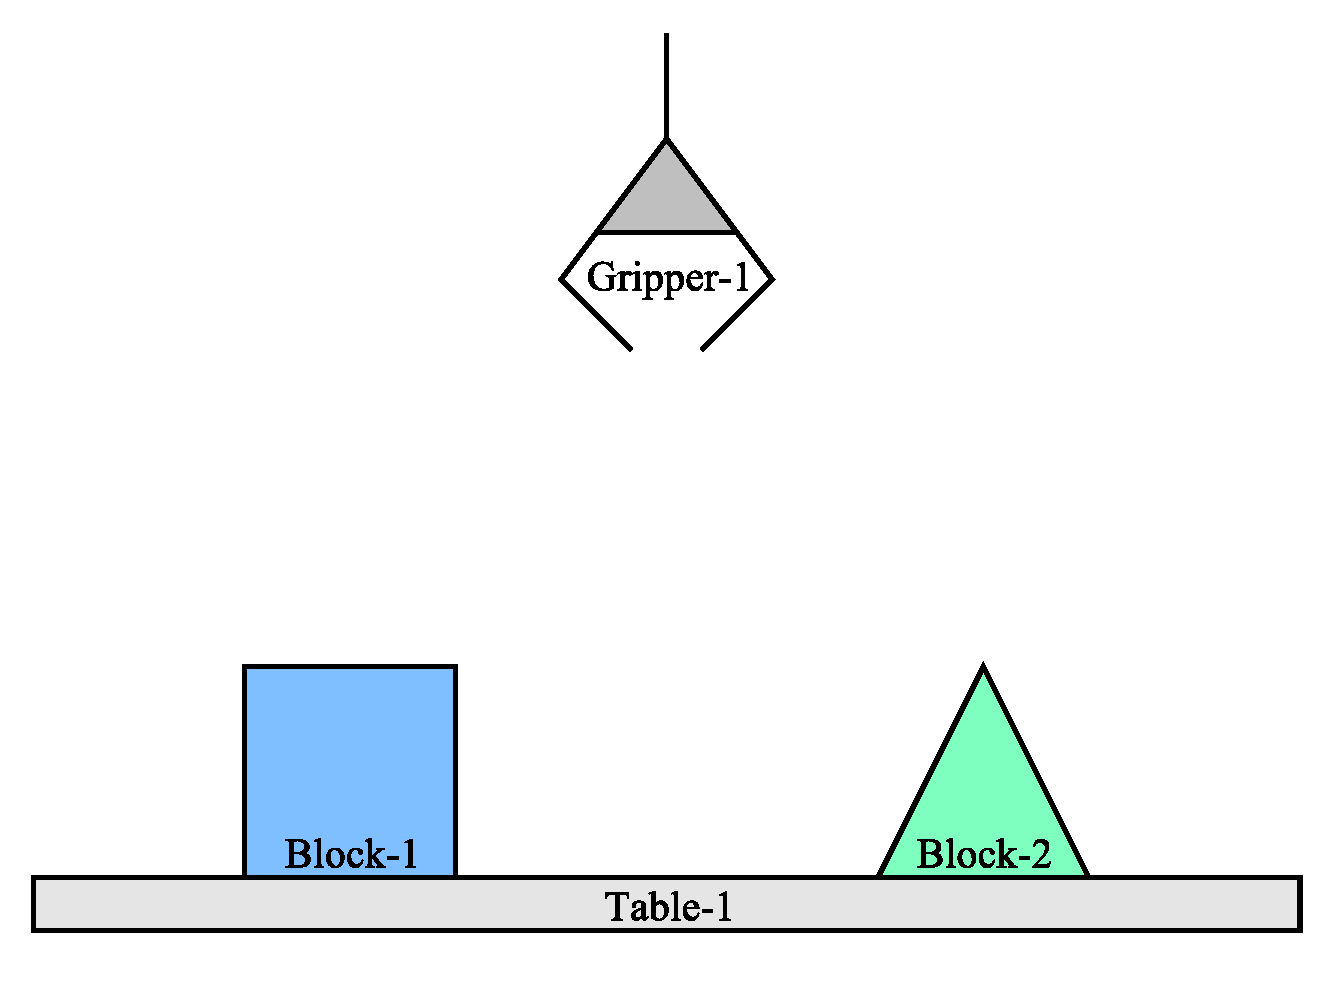
\includegraphics[width=8cm]{gfx/blocks_world_example-1}
\end{center}
\caption[An example problem domain.]{An example problem domain.}
\label{figure:an_example_problem_domain}
\end{figure}
\begin{sidewaysfigure}
\begin{center}
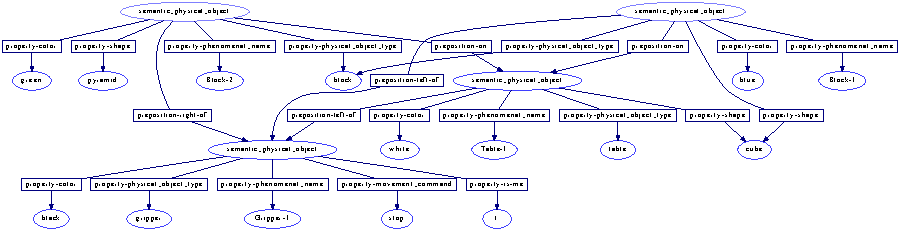
\includegraphics[width=24cm]{gfx/implemented_physical_knowledge}
\end{center}
\hspace{4cm}\parbox{15cm}{\caption[The physical knowledge-base.]{The
    physical
    knowledge-base.}\label{figure:implemented_physical_knowledge}}
\end{sidewaysfigure}

\section{Procedurally Reflective Event Stream}



\section{Abstraction}



\section{An Example Storyboard}

{\mbox{\autoref{figure:implemented_example_learning_storyboard}}}
shows a storyboard of the implemented example of second-order
learning.
\begin{figure}
\begin{center}
\begin{tabular}{p{4cm}p{4cm}p{4cm}}
1. 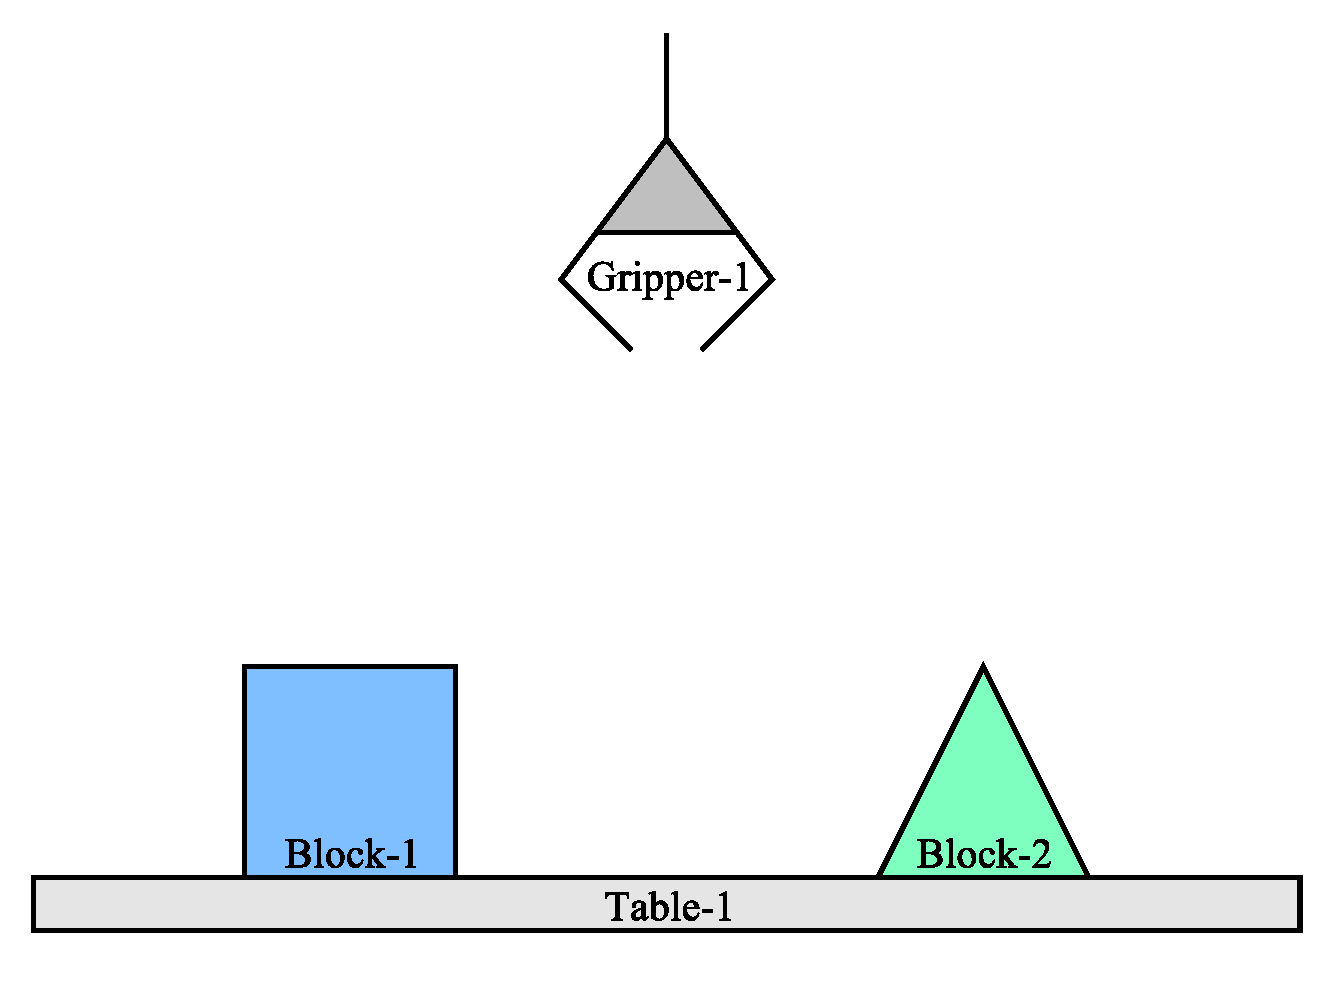
\includegraphics[width=4cm]{gfx/blocks_world_example-1}  & 2. 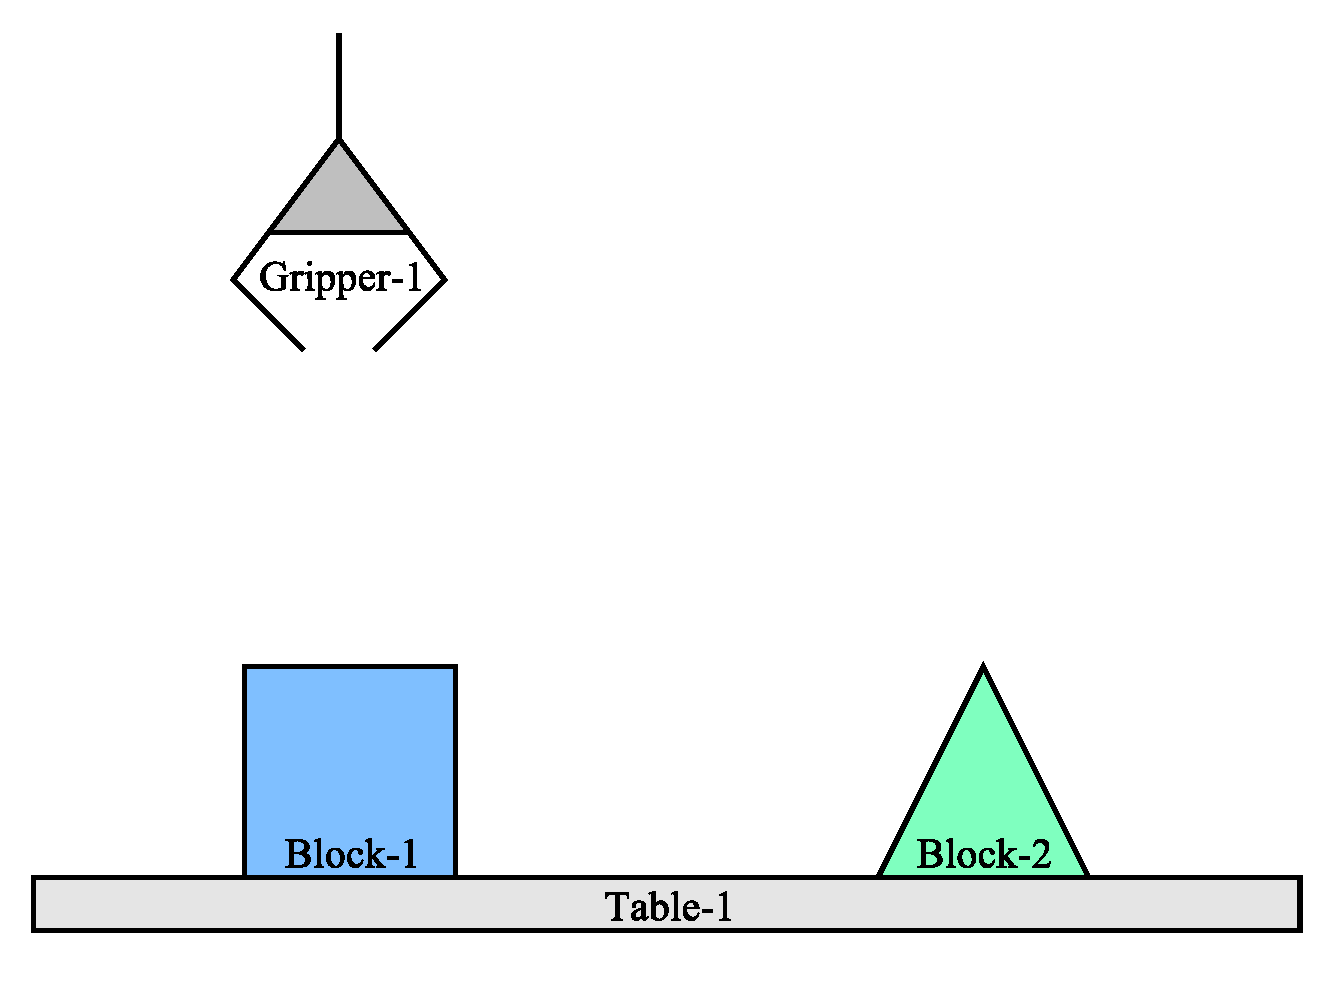
\includegraphics[width=4cm]{gfx/blocks_world_example-2}  & 3. 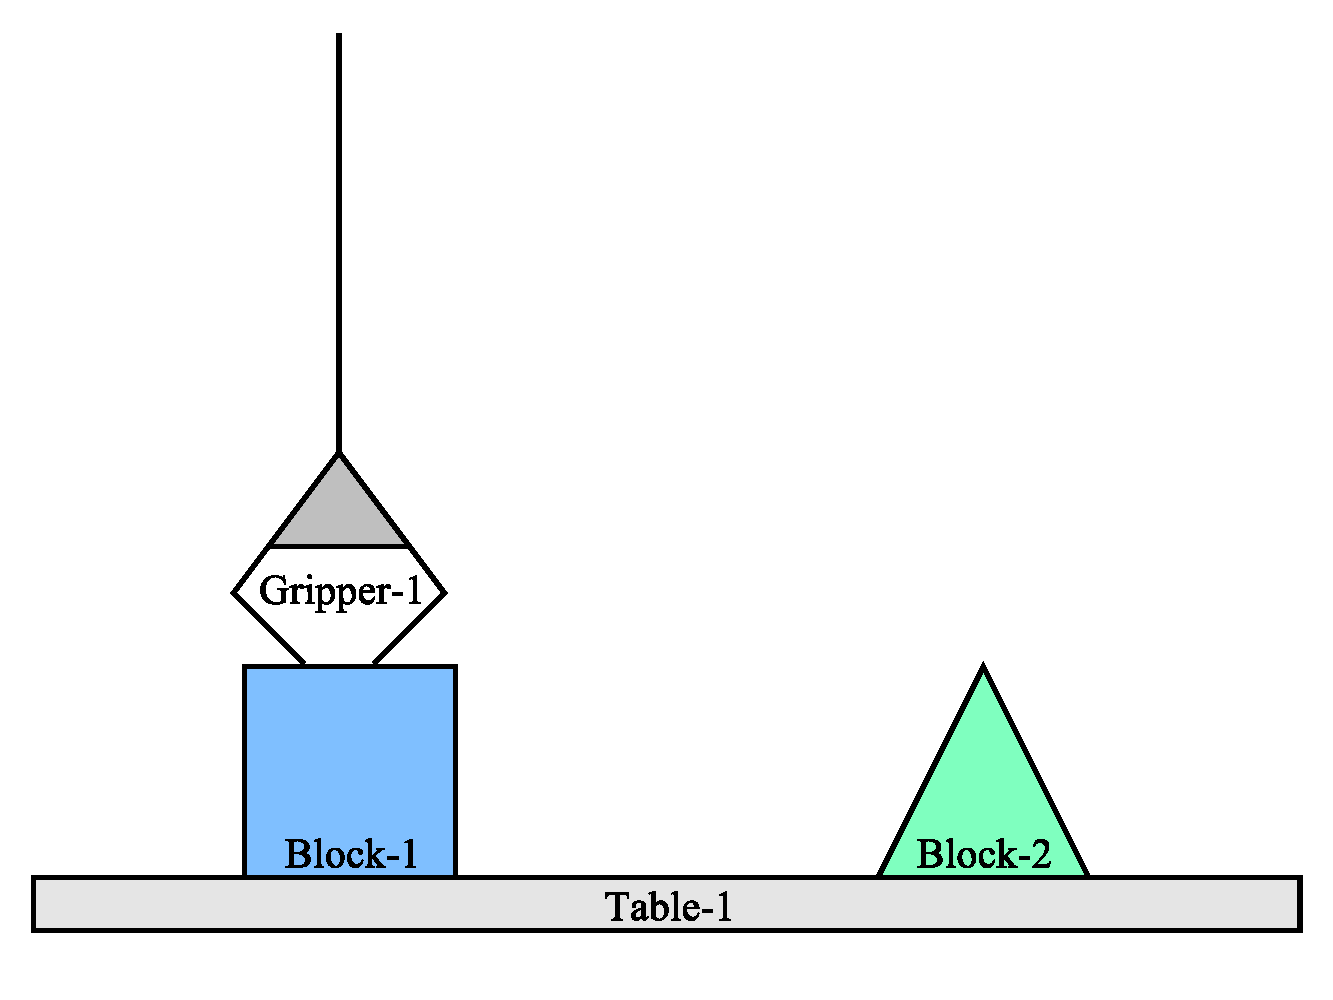
\includegraphics[width=4cm]{gfx/blocks_world_example-3} \\
4. 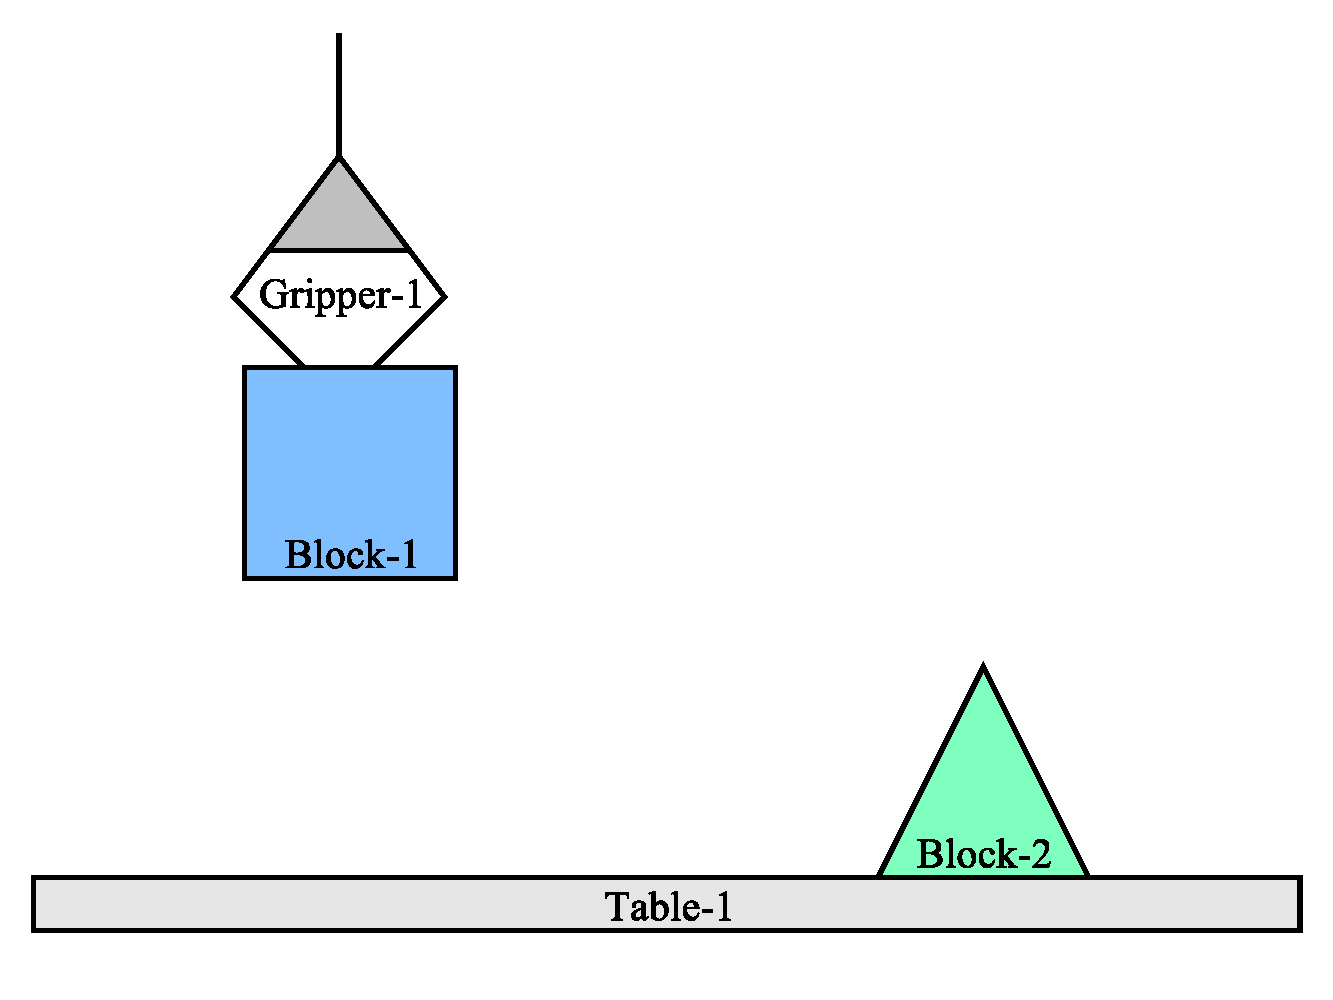
\includegraphics[width=4cm]{gfx/blocks_world_example-4}  & 5. 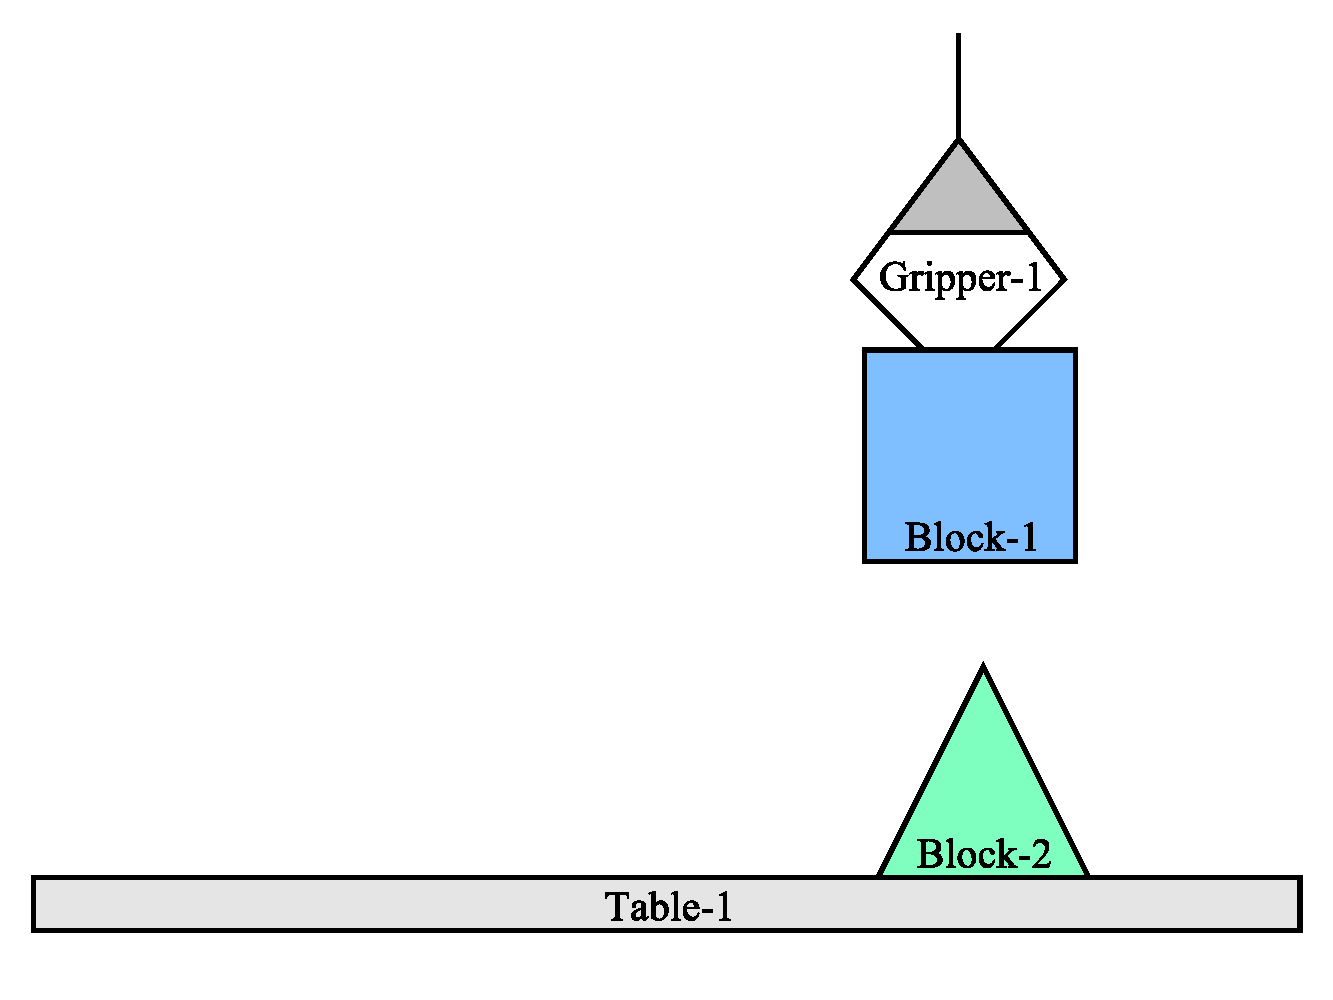
\includegraphics[width=4cm]{gfx/blocks_world_example-5}  & 6. 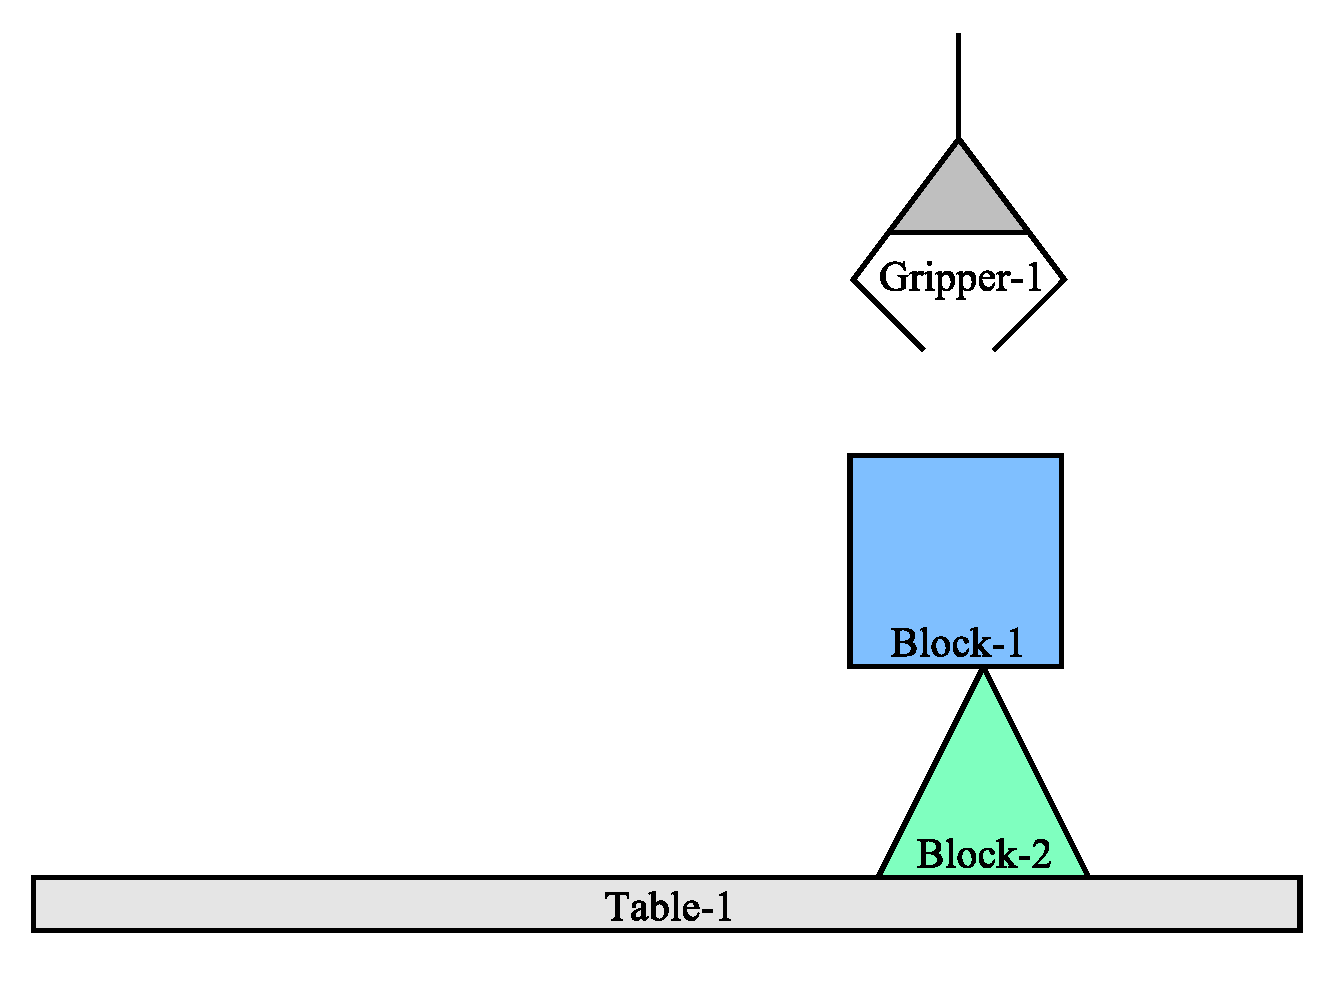
\includegraphics[width=4cm]{gfx/blocks_world_example-6} \\
7. 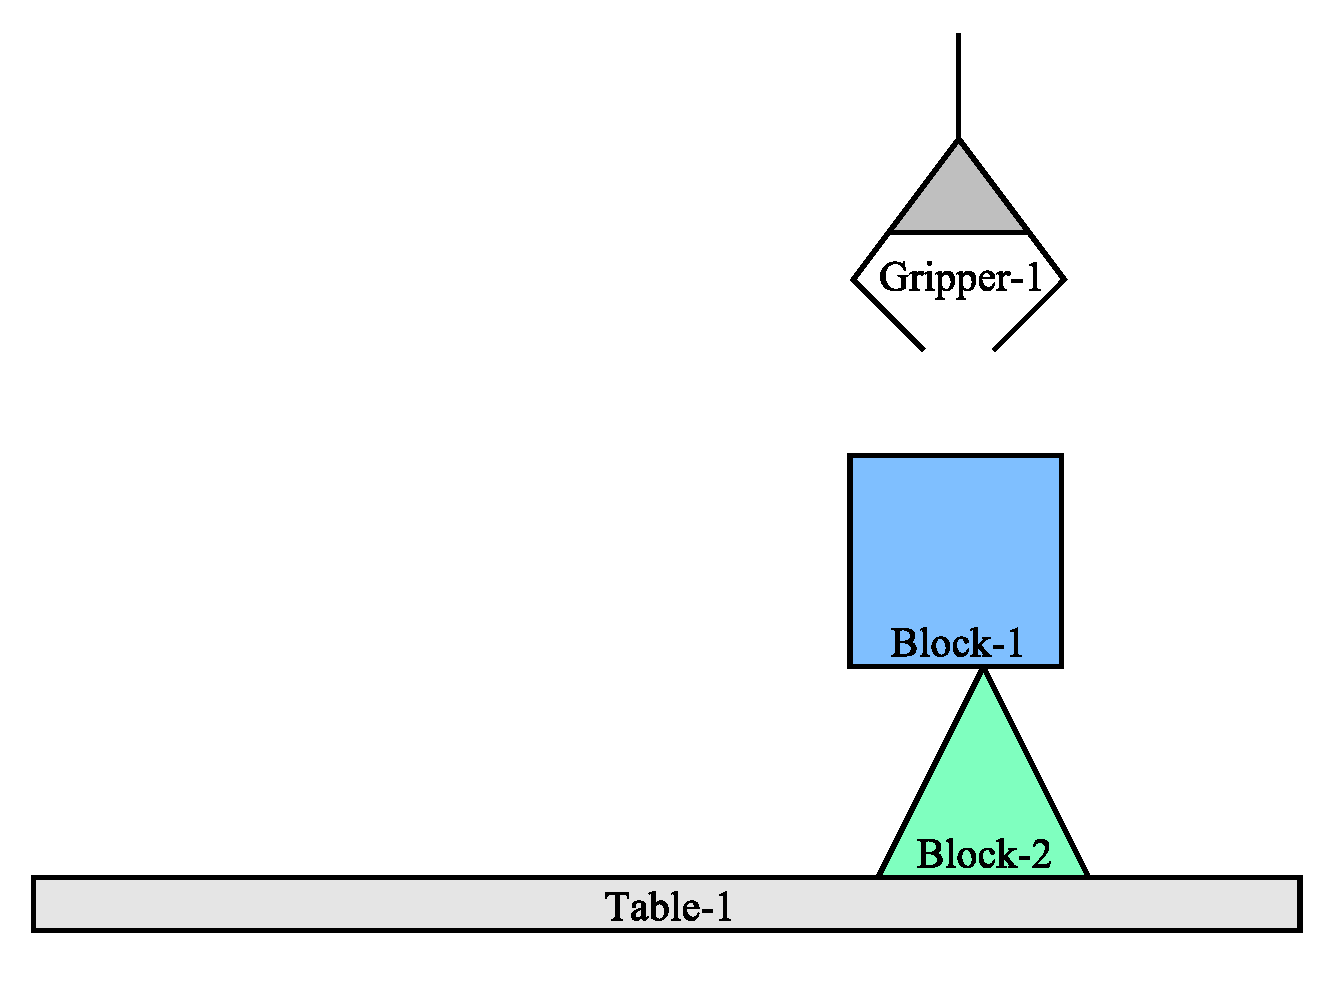
\includegraphics[width=4cm]{gfx/blocks_world_example-7}  & 8. 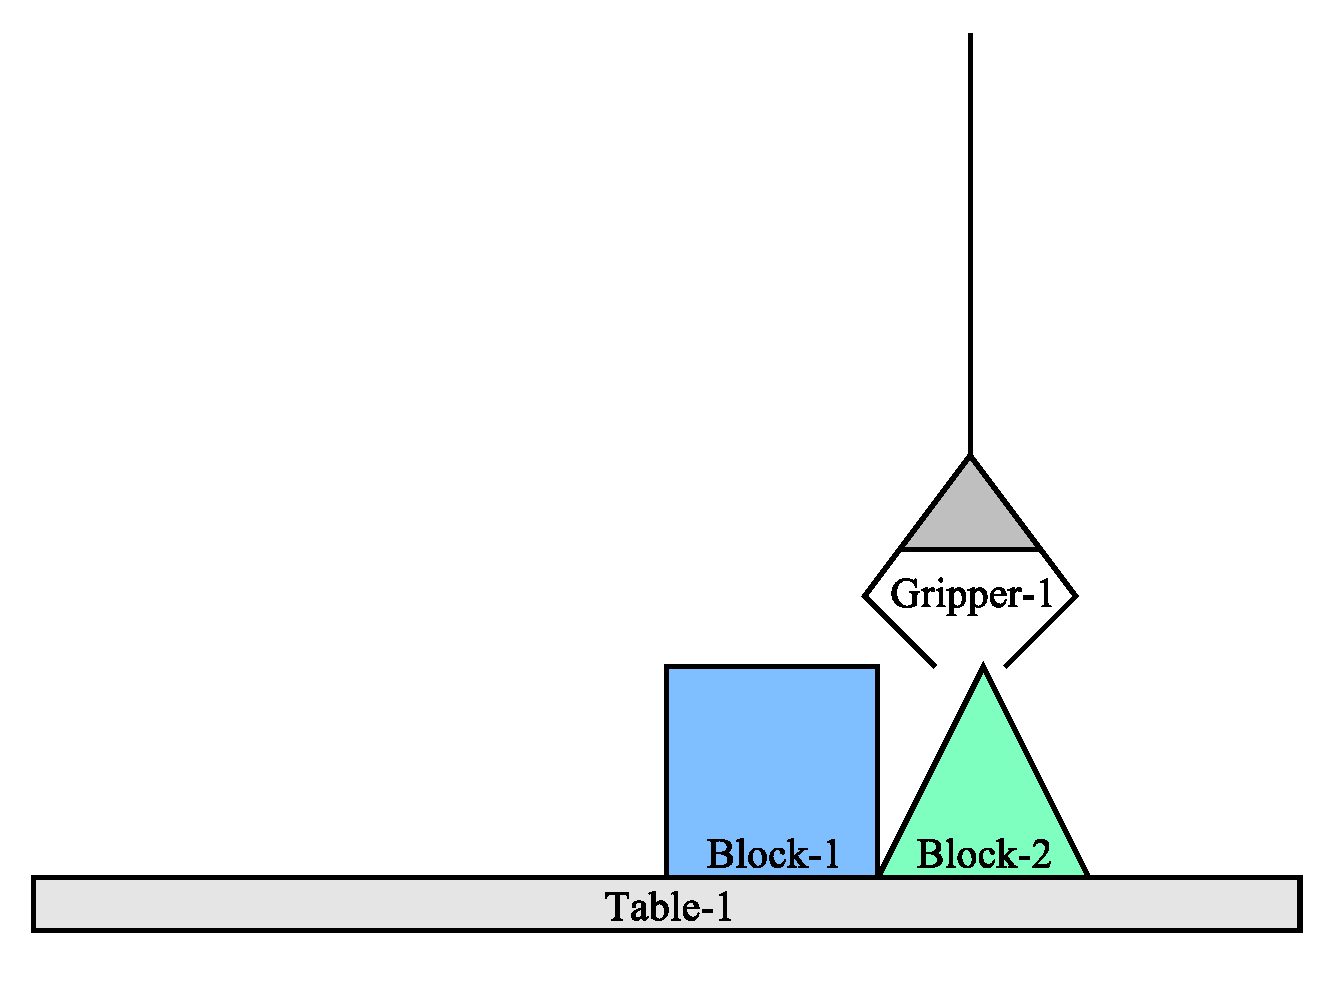
\includegraphics[width=4cm]{gfx/blocks_world_example-8}  & 9. 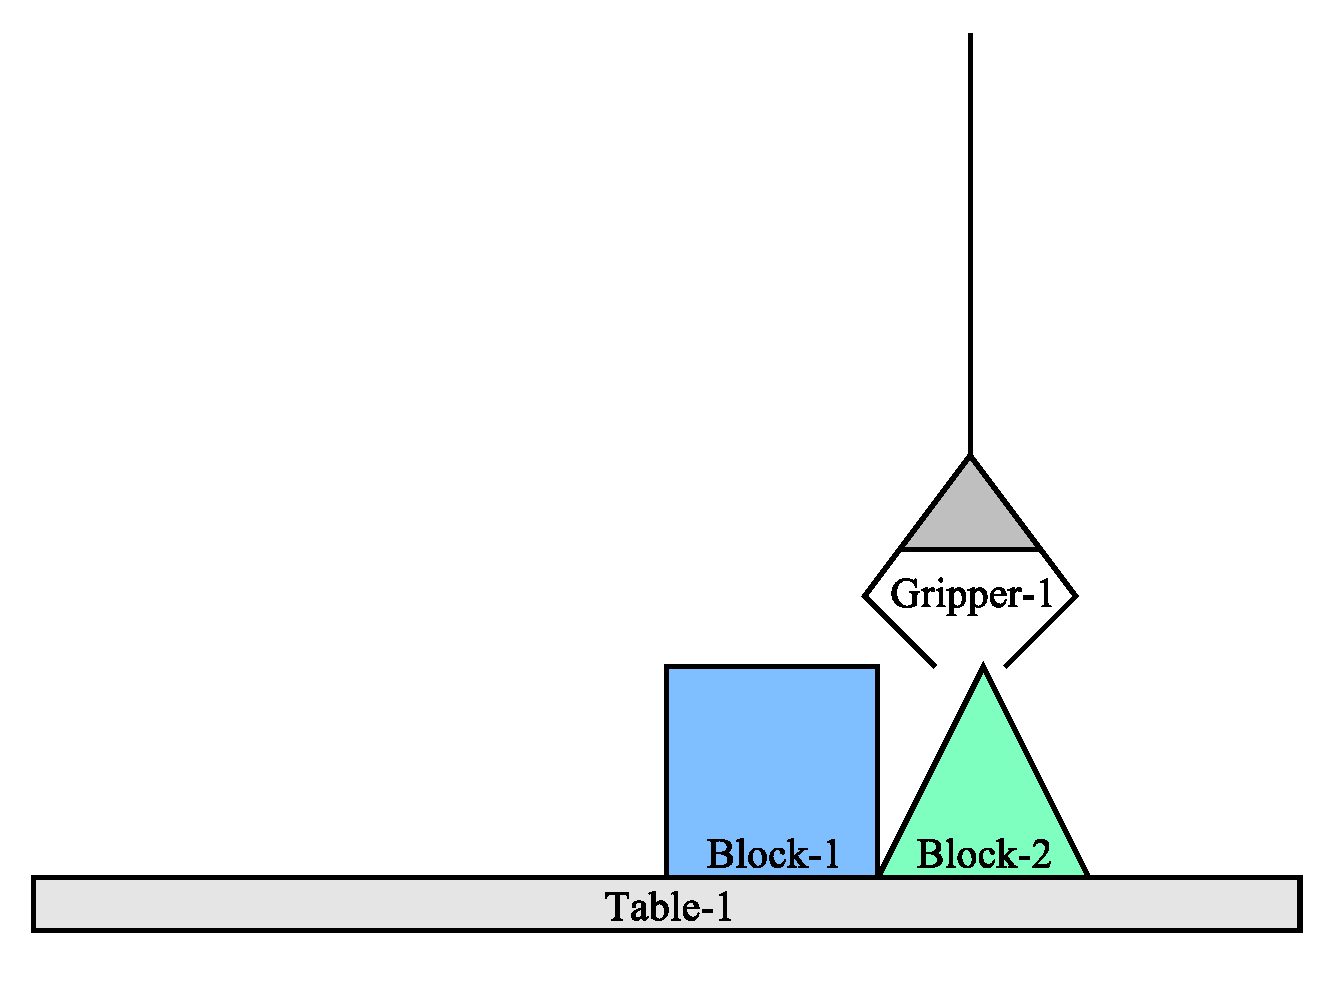
\includegraphics[width=4cm]{gfx/blocks_world_example-9} \\
10. 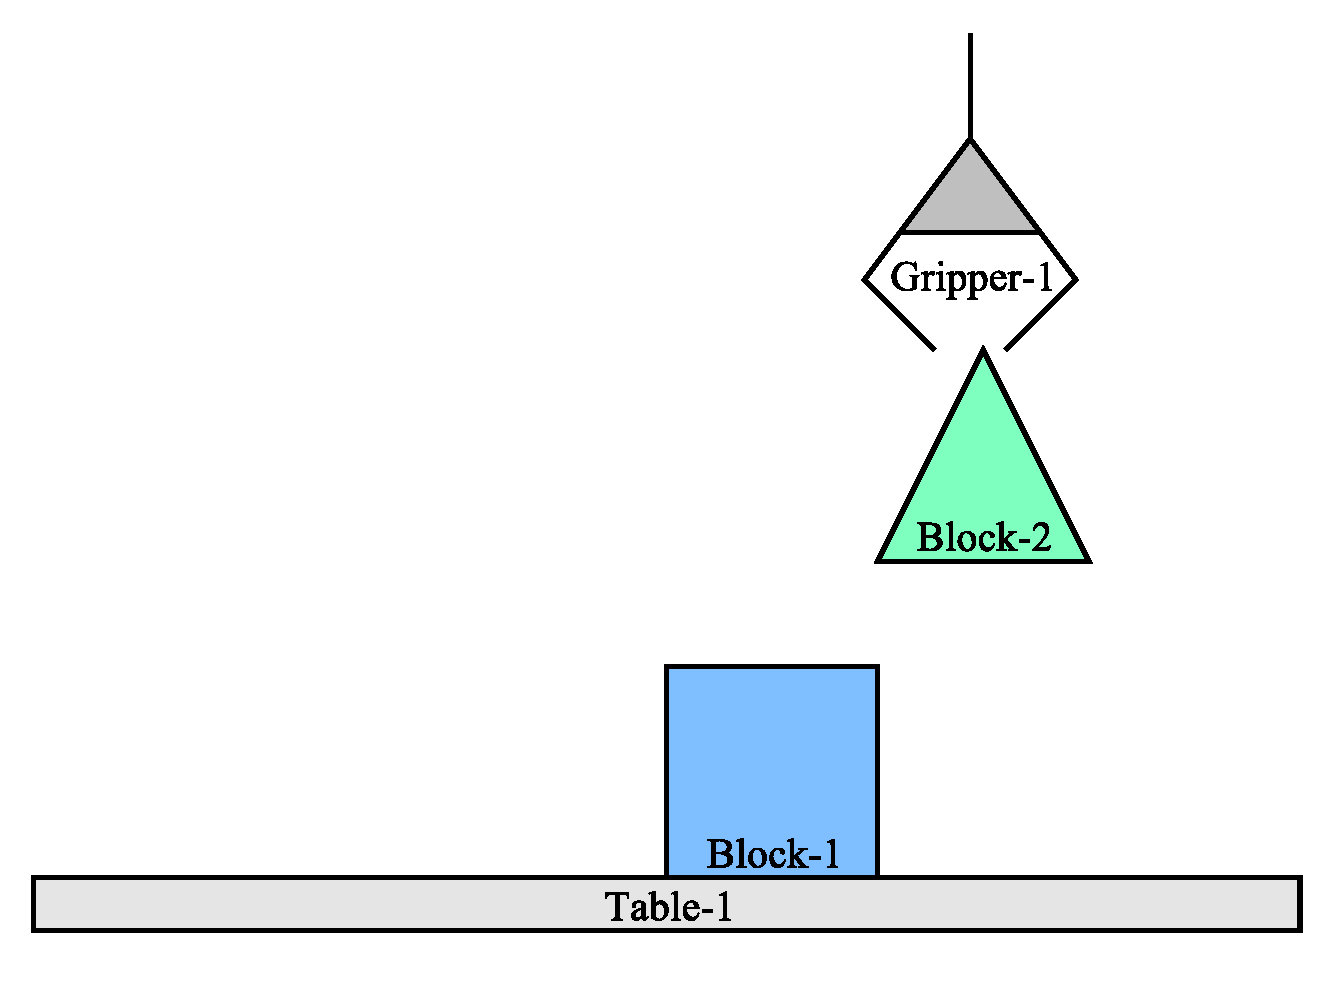
\includegraphics[width=4cm]{gfx/blocks_world_example-10} & 11. 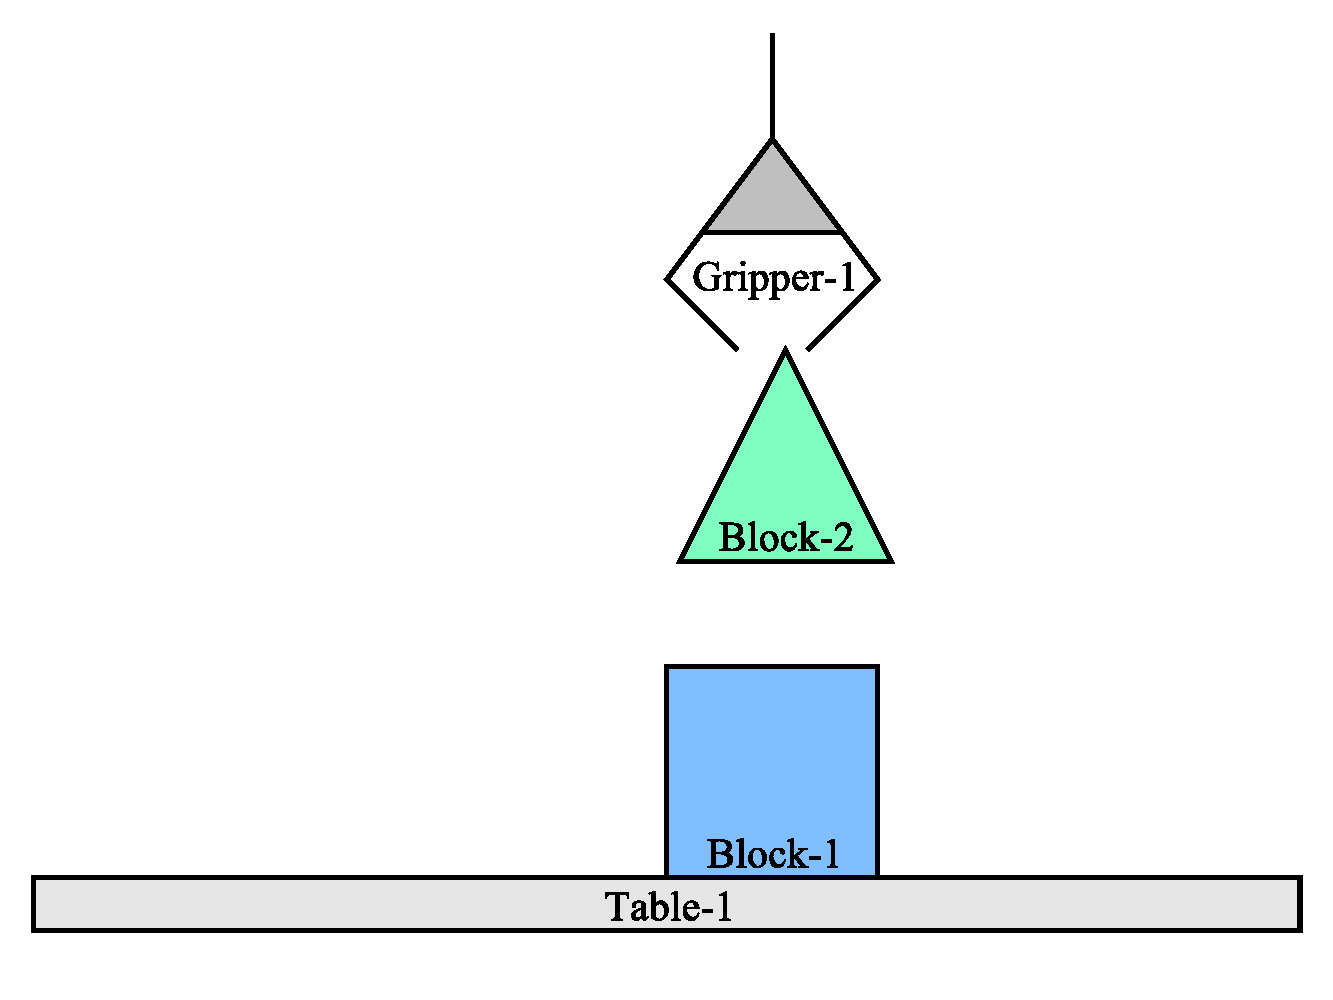
\includegraphics[width=4cm]{gfx/blocks_world_example-11} & 12. 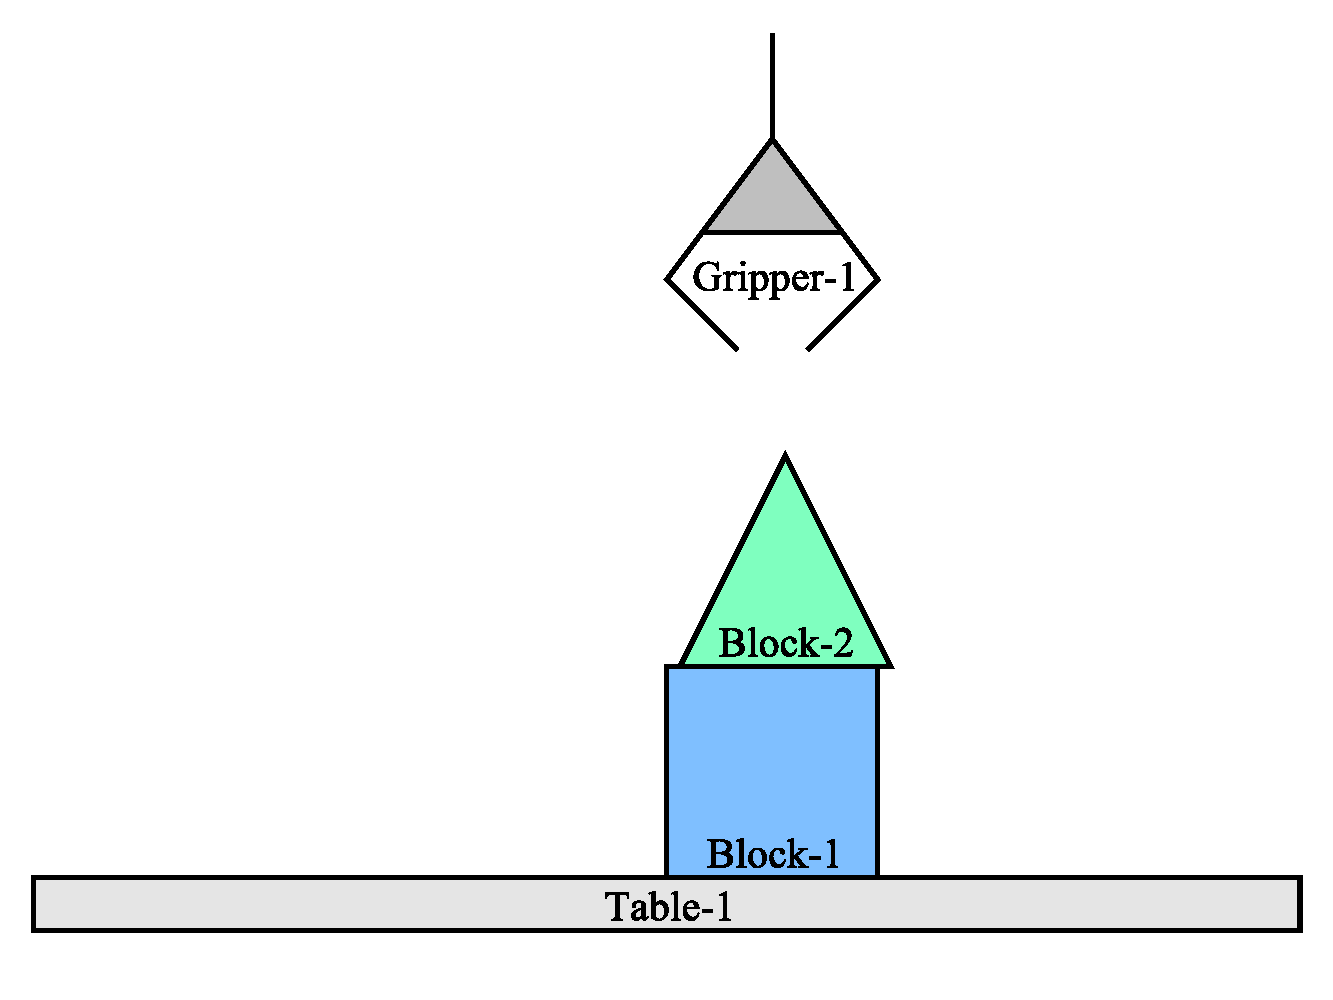
\includegraphics[width=4cm]{gfx/blocks_world_example-12}
\end{tabular}
\end{center}
\caption[A storyboard of the implemented example of second-order
  learning.]{A storyboarded example of second-order learning, where
  the goal is to create a stack of two blocks.  (1) A plan that is
  hypothesized to stack the square block on top of the triangular
  block is executed.  (2--8) The plan completes execution and results
  in the square falling off of the triangle, an expectation failure.
  (9) The second-order hypothetical heuristic is learned that predicts
  plan failure will result by executing plans that try to stack
  squares on top of triangles.  A plan that is hypothesized to stack
  the triangle on top of the square is executed.  (9-12) The second
  plan completes execution, accomplishing the physical goal.}
\label{figure:implemented_example_learning_storyboard}
\end{figure}

